\documentclass[11pt]{article}

\usepackage[margin=1in]{geometry}
\usepackage{amsmath,amssymb}
\usepackage{booktabs}
\usepackage{graphicx}
\usepackage[numbers,sort&compress]{natbib}
\usepackage{hyperref}

\title{Supplementary Material: Background-Guided Residual Flow Matching for Multi-Constraint Seismic Velocity Model Building}
\author{[Same author list as main manuscript]}
\date{}

\begin{document}
\maketitle

\section{S1. Extended Condition-Learning and Residual Objectives}

Let $a_{i,m}\in\{0,1\}$ denote modality availability, $q_{i,m}\in[0,1]$ externally supplied quality, and $r_{i,m}^{k}$ learned reliability for role $k\in\{\mathrm{bg},\mathrm{str}\}$. The role-specific fusion weights are
\begin{equation}
\widetilde w_{i,m}^{k}=a_{i,m}q_{i,m}r_{i,m}^{k},
\qquad
w_{i,m}^{k}=
\frac{\widetilde w_{i,m}^{k}}
{\max\left(\sum_{m'}\widetilde w_{i,m'}^{k},10^{-6}\right)}.
\end{equation}
Unavailable modalities therefore receive zero weight, while the weights over observed modalities remain normalized.

Training-only Haar anchors calibrate the background and structural role spaces. Subset-aware multimodal alignment, symmetric anchor calibration, cross-role separation, and reliability regularization form the condition objective
\begin{equation}
\mathcal L_C=
\mathcal L_{\mathrm{subsym}}^{\mathrm{bg}}
+\mathcal L_{\mathrm{subsym}}^{\mathrm{str}}
+\lambda_A\mathcal L_A
+\lambda_{\mathrm{bg,str}}\mathcal L_{\mathrm{bg,str}}^{\perp}
+\lambda_{\mathrm{aux}}\mathcal L_{\mathrm{aux}}^{\perp}
+\lambda_Q\mathcal L_{\mathrm{rel}}.
\end{equation}
These target-derived anchors are used only during training and never cross the observed-only inference boundary.

For the residual branch, the endpoint reconstruction objective supplements Flow Matching:
\begin{align}
\widetilde R
&=R_t+(1-t)v_\theta(R_t,t,c),\\
\mathcal L_R
&=\mathcal L_{\mathrm{FM}}
+\lambda_{\mathrm{rec}}\|\bar B+\widetilde R-V\|_1
+\lambda_L\|P_L(\widetilde R)-P_L(R_{\hat B})\|_1.
\end{align}
The low-pass term matches the actual prediction-relative residual target rather than forcing the residual to be purely high frequency.

\section{S2. Effective-Rank Characterization}

For a decomposition $V=B+S$, with $B=P_L(V)$ and $S=V-B$, the participation-ratio effective rank is
\begin{equation}
r_{\mathrm{eff}}=
\frac{\left(\sum_j\lambda_j\right)^2}{\sum_j\lambda_j^2},
\end{equation}
where $\{\lambda_j\}$ are nonzero covariance eigenvalues. The analysis uses 1,000 fixed training records per OpenFWI subset. No learned dimensionality reducer or checkpoint enters the calculation.

\begin{table}[t]
\centering
\caption{Participation-ratio effective rank of the background and structural complement.}
\begin{tabular}{lrr}
\toprule
Subset & Background $B$ & Structure $S$ \\
\midrule
FlatVel-A & 2.02 & 24.26 \\
FlatVel-B & 5.66 & 39.67 \\
CurveVel-A & 2.59 & 58.52 \\
CurveVel-B & 7.53 & 200.89 \\
FlatFault-A & 3.06 & 37.83 \\
FlatFault-B & 7.54 & 289.69 \\
CurveFault-A & 4.24 & 49.54 \\
CurveFault-B & 10.54 & 407.91 \\
\midrule
Median & 4.95 & 54.03 \\
\bottomrule
\end{tabular}
\end{table}

The structural complement has higher effective rank in every subset. In the journal manuscript this is treated as a data-level characterization that motivates distinct reconstruction roles, not as a proof of lower conditional entropy or guaranteed learnability.

\section{S3. Missing-Modality Stress Tests}

A fixed historical BG-RFM checkpoint was evaluated without retraining under several observation-removal settings. RMS velocity is part of the standard benchmark observation contract; RMS-missing rows are therefore stress tests rather than the intended operating scenario.

\begin{table}[t]
\centering
\caption{Historical missing-modality stress test without retraining or test-time adaptation.}
\begin{tabular}{lrrr}
\toprule
Observation subset & MAE & RMSE & SSIM \\
\midrule
Full input & 0.0150 & 0.0269 & 0.9915 \\
w/o well log & 0.0168 & 0.0295 & 0.9899 \\
w/o horizon & 0.1011 & 0.1669 & 0.8202 \\
w/o RMS velocity & 0.3947 & 0.4705 & 0.0753 \\
w/o well log + RMS velocity & 0.4684 & 0.5303 & 0.0192 \\
PoSTM only & 0.4706 & 0.5356 & 0.0154 \\
\bottomrule
\end{tabular}
\end{table}

The modest change after removing wells contrasts with the much larger degradation after removing horizon or RMS information. The result supports complementarity among the constraints but is not interpreted as a field-robustness guarantee.

\section{S4. Additional Design Controls and Diagnostics}

The original experimental package contains controls that complement the main design table: direct residual regression, removal of the condition objective, uniform role fusion, and oracle-background diagnostics. These controls were used to inspect specific mechanisms but are not all required in the main article.

For the residual transport diagnostic, with $d=HW$,
\begin{equation}
q_T=
\frac{d^{-1}\|V-\hat B\|_2^2+1}
{d^{-1}\|V\|_2^2+1}.
\end{equation}
All 33,600 held-out samples satisfy $q_T<1$ in the retained analysis; the mean is 0.772 with bootstrap 95\% confidence interval $[0.771,0.773]$. This quantifies the straight-path target-energy change in the stated normalized coordinates. It is reported as a diagnostic observation rather than a causal theorem.

\begin{figure}[t]
\centering
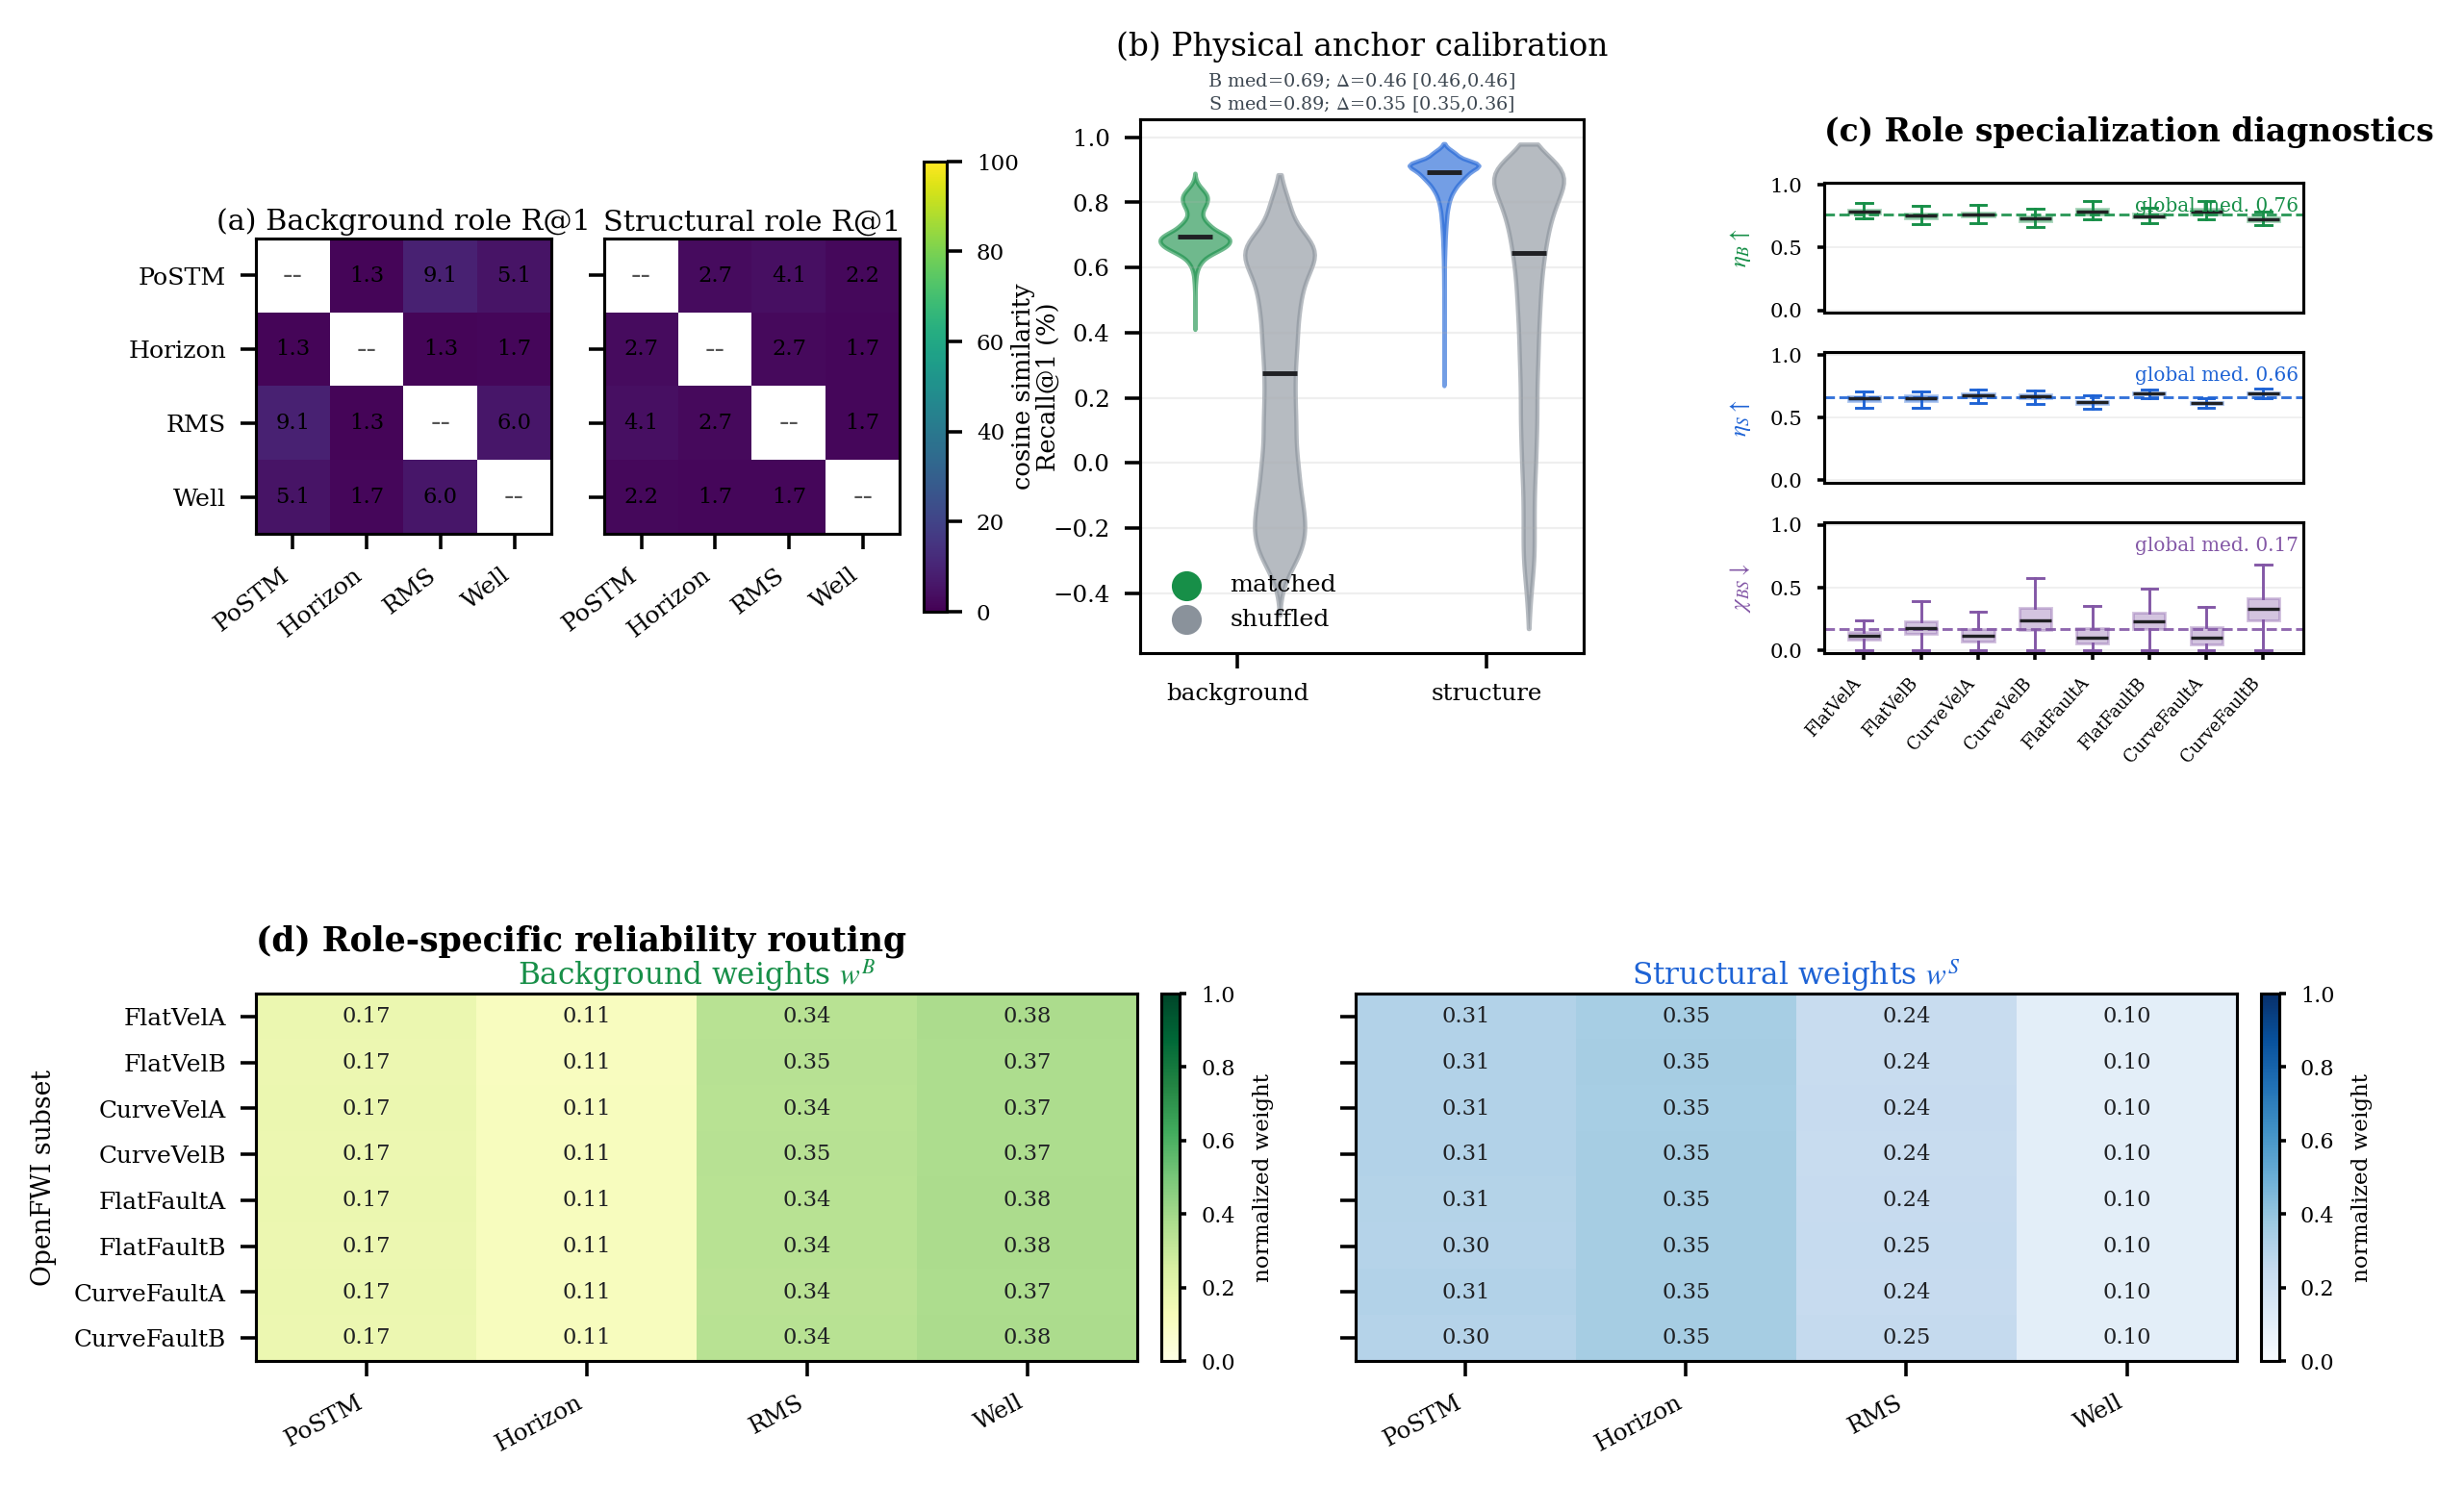
\includegraphics[width=0.95\textwidth]{../AAAI2027/figures/figure3_condition_learning/appendix_full_condition_diagnostics.png}
\caption{Extended condition-routing diagnostics retained from the completed experimental package.}
\end{figure}

\section{S5. Baseline Adaptation and Parameter Accounting}

The journal's main comparison uses matched-input adaptations so that all evaluated estimators receive the same multimodal observations and held-out membership. The rows should therefore be interpreted as controlled estimator comparisons, not as source-native reproductions.

\begin{itemize}
    \item \textbf{InversionNet adaptation:} the encoder--decoder capacity is adapted to the multimodal input and trained with supervised velocity reconstruction.
    \item \textbf{VelocityGAN adaptation:} multimodal input is used while retaining adversarial plus reconstruction training.
    \item \textbf{UPFWI adaptation:} the implementation is a supervised multimodal estimator and is explicitly labeled as such; it is not the original unsupervised/physics-coupled UPFWI protocol.
    \item \textbf{Latent U-Net adaptation:} the latent U-Net architecture is adapted to the common multimodal translation task.
\end{itemize}

The main-table parameter counts are 24.41M for InversionNet, 25.59M for VelocityGAN, approximately 19.00M for the supervised multimodal UPFWI adaptation, 35.12M for Latent U-Net, and 10.60M for BG-RFM. Parameter count is reported as model compactness and is not used as a substitute for runtime.

\section{S6. Extended Qualitative Evidence}

The completed AAAI-era package retained fixed-rule representative cases as well as explicit advantage and failure-case panels. These are useful for checking whether the visual interpretation is restricted to favorable examples.

\begin{figure}[t]
\centering
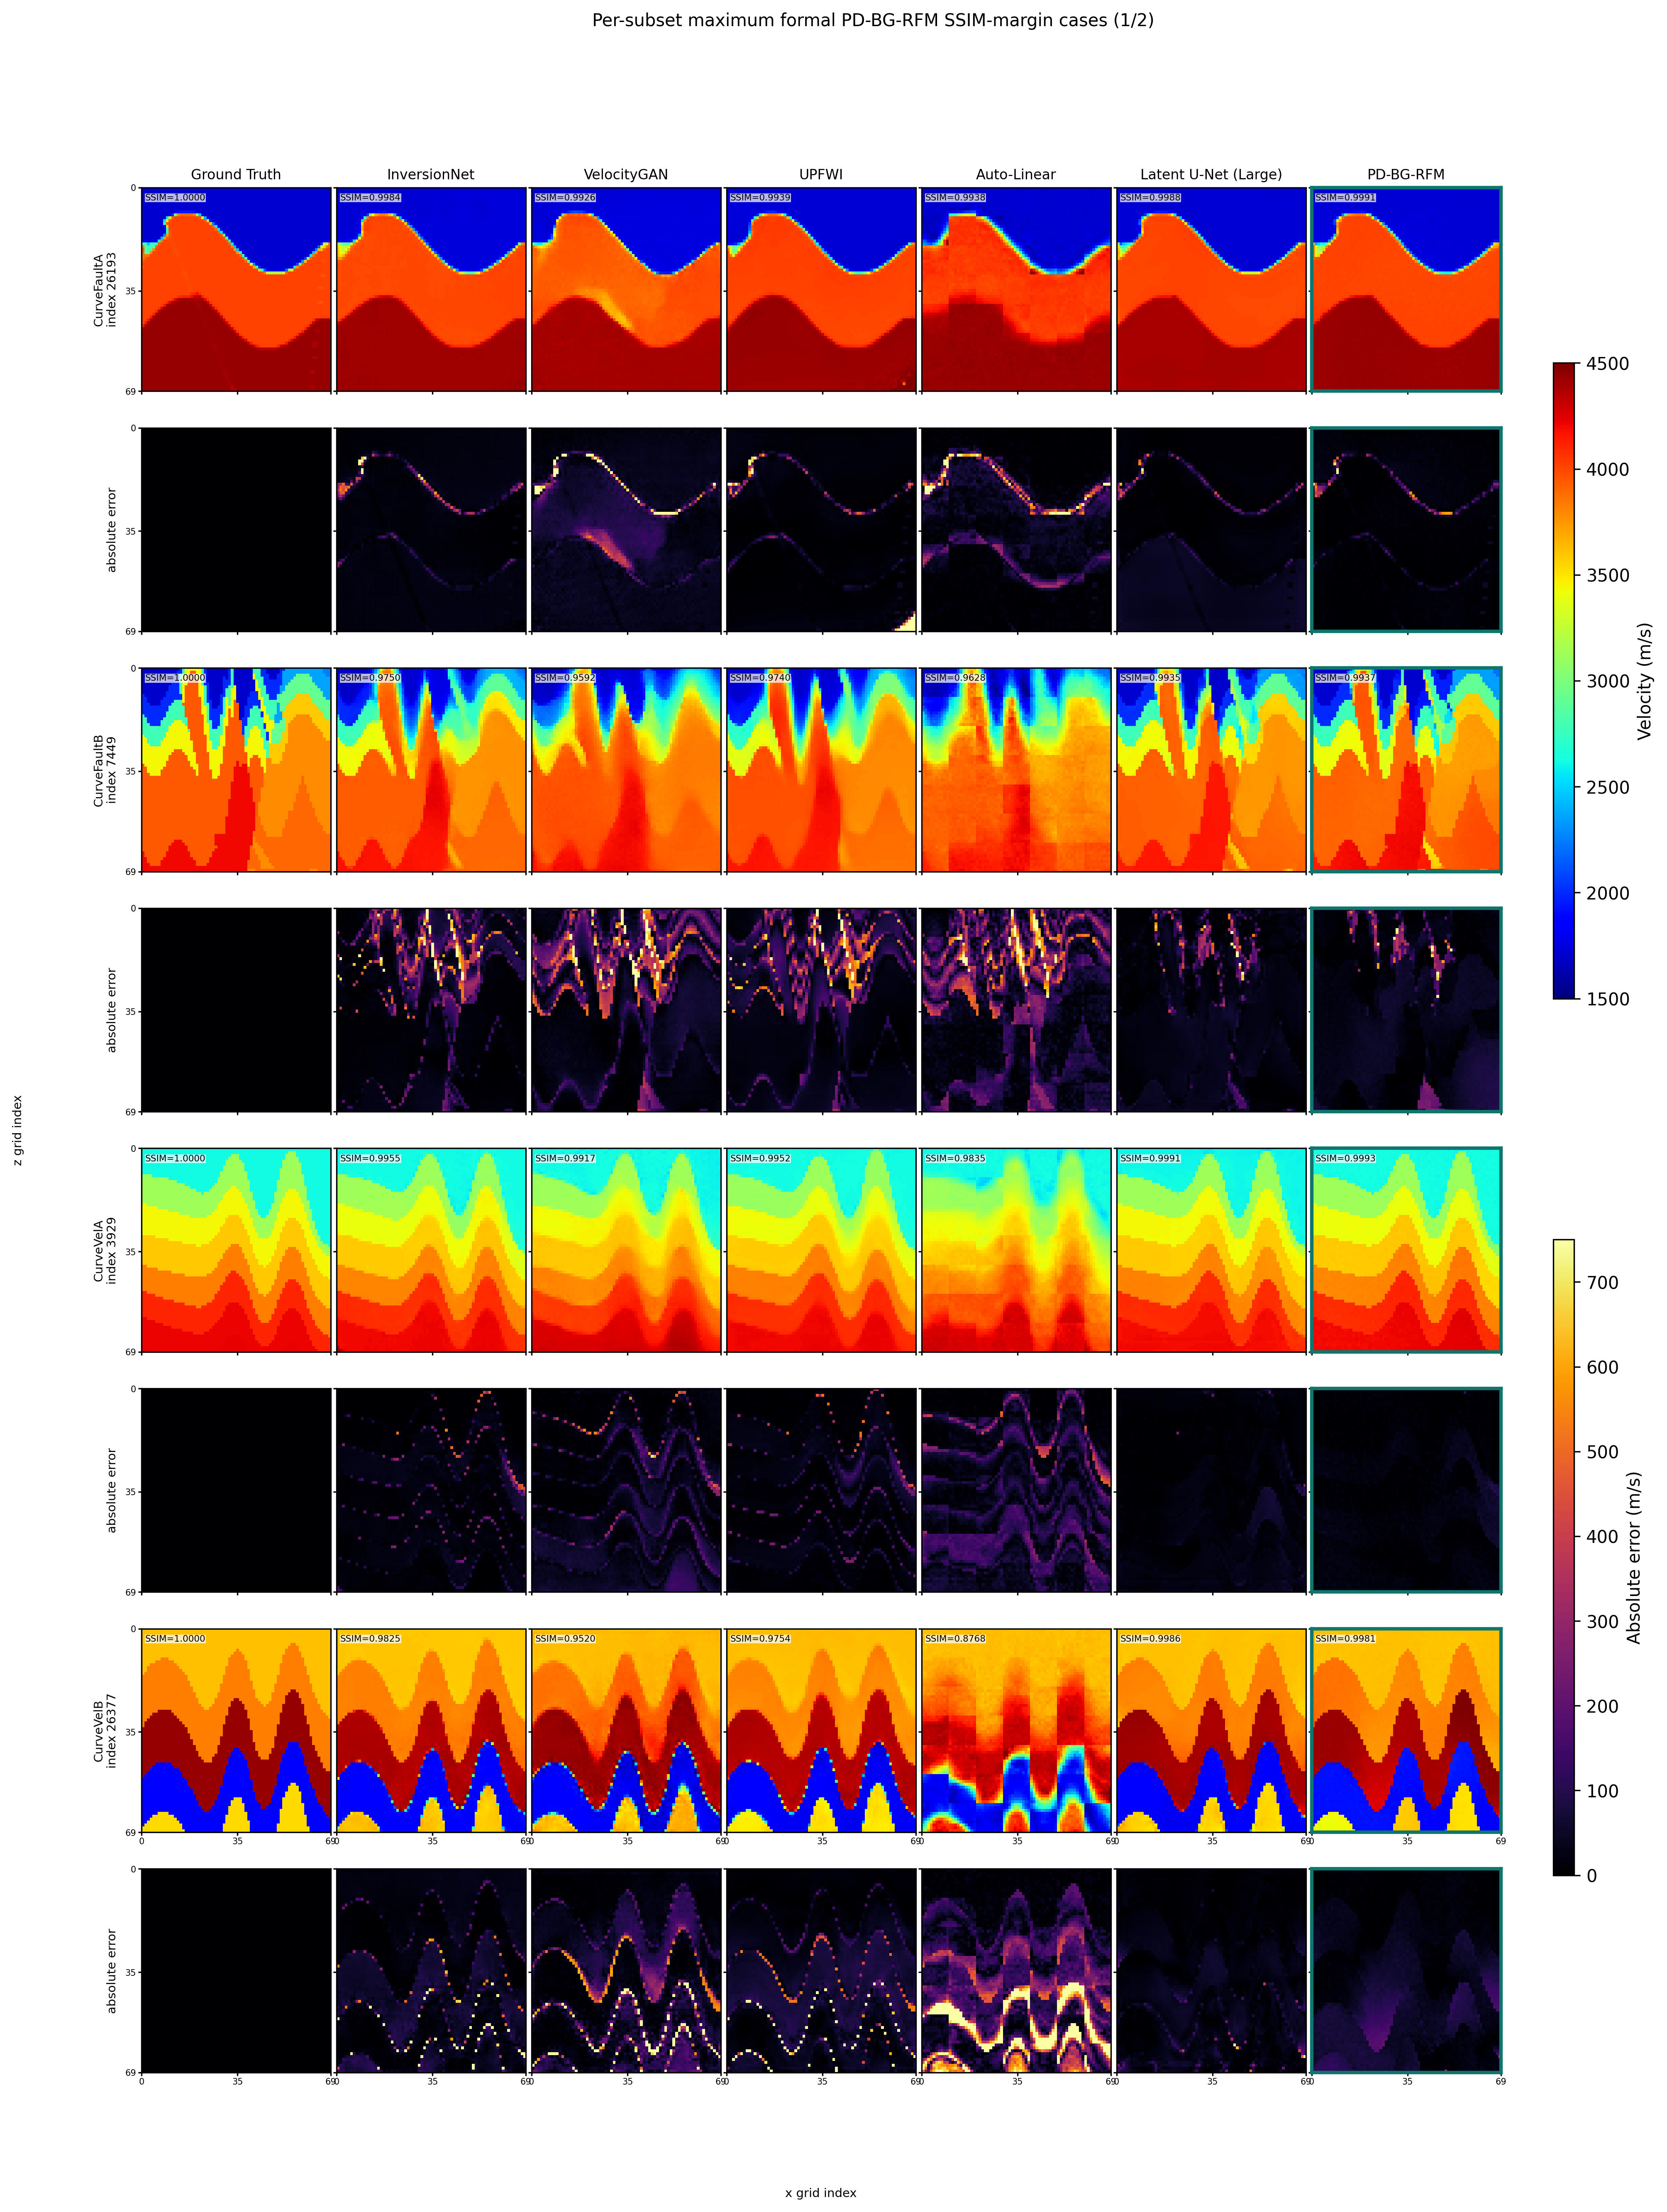
\includegraphics[width=0.98\textwidth]{../AAAI2027/figures/table2_qualitative/table2_representative_cases_1.png}
\caption{Extended representative held-out cases, part I.}
\end{figure}

\begin{figure}[t]
\centering
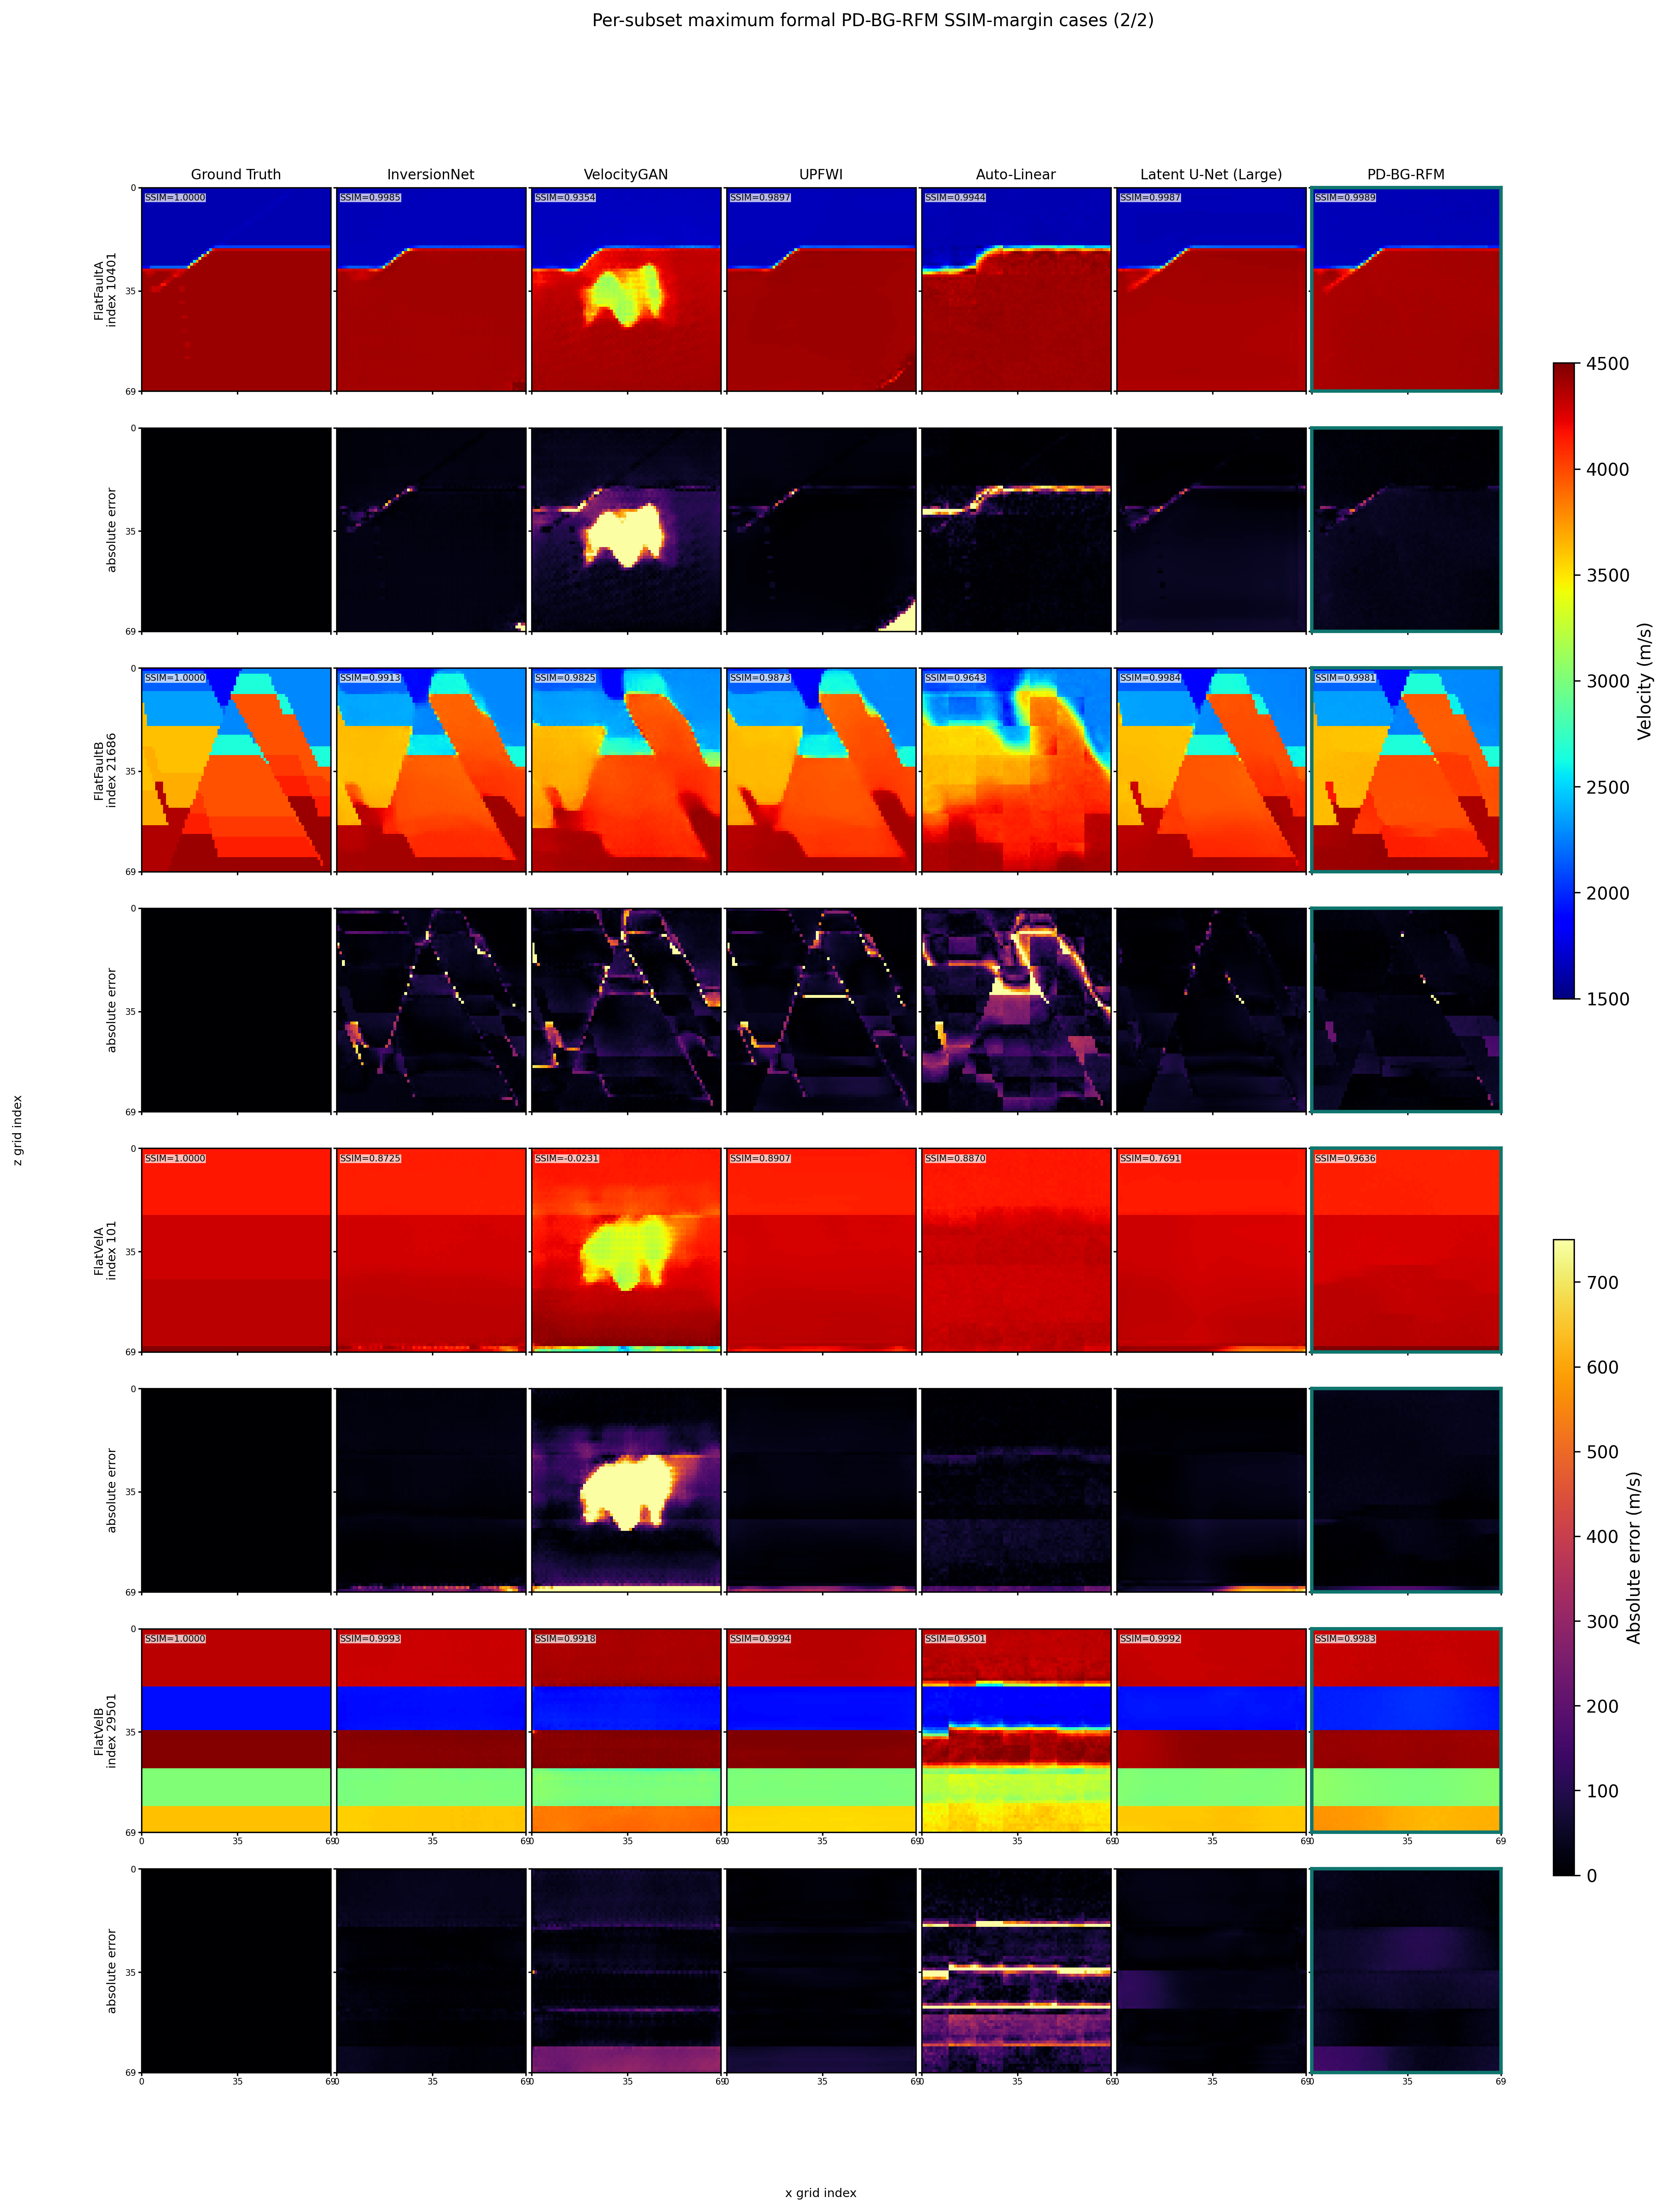
\includegraphics[width=0.98\textwidth]{../AAAI2027/figures/table2_qualitative/table2_representative_cases_2.png}
\caption{Extended representative held-out cases, part II.}
\end{figure}

\begin{figure}[t]
\centering
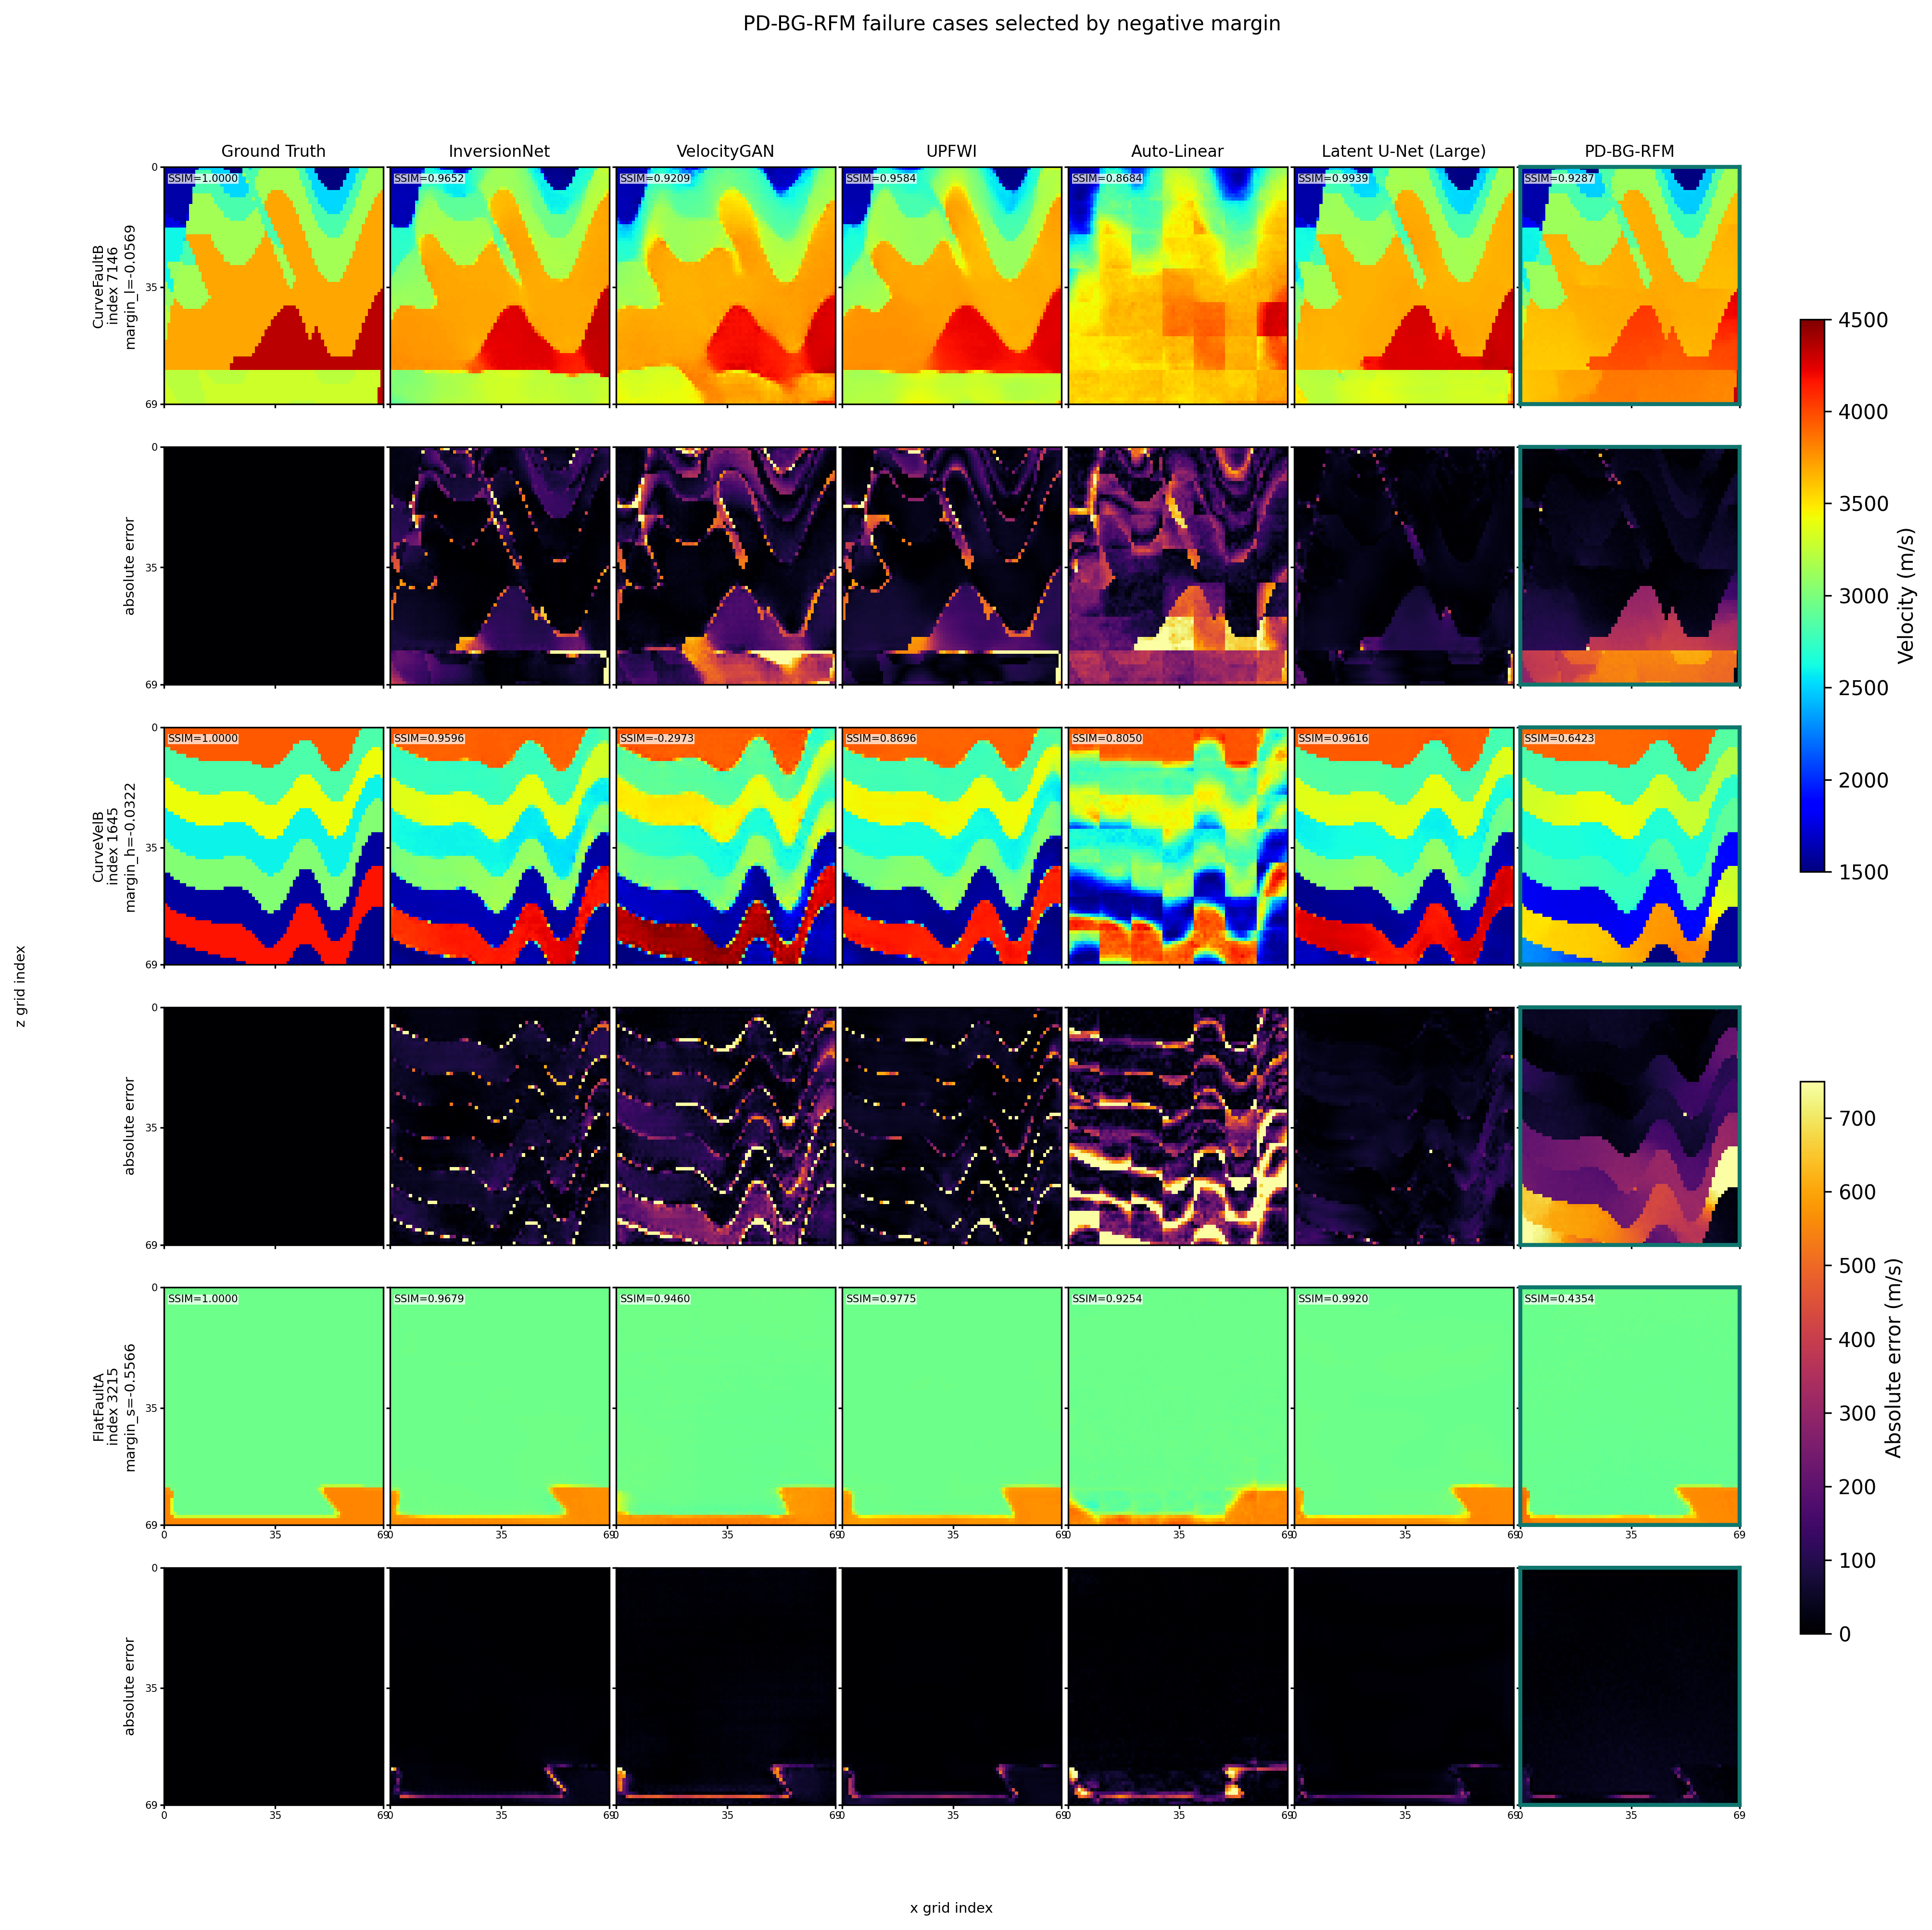
\includegraphics[width=0.98\textwidth]{../AAAI2027/figures/table2_qualitative/table2_failure_cases.png}
\caption{Retained failure-case panel from the historical matched-input qualitative analysis.}
\end{figure}

\bibliographystyle{unsrtnat}
\bibliography{references}

\end{document}
